\documentclass[10pt,conference]{IEEEtran}

\ifCLASSINFOpdf
	\usepackage[pdftex]{graphicx}
	%\graphicspath{{./figs/}}
	\DeclareGraphicsExtensions{.pdf,.jpeg,.png}
\else
	\usepackage[dvips]{graphicx}
	%\graphicspath{{./figs/}}
	\DeclareGraphicsExtensions{.eps}
\fi

\usepackage[cmex10]{amsmath}
\usepackage[tight,footnotesize]{subfigure}
\usepackage{xcolor}
\usepackage[lined,ruled]{algorithm2e}

\usepackage[latin1]{inputenc}
\usepackage{tikz}
\usetikzlibrary{shapes}
\usetikzlibrary{arrows}

\usepackage[]{algorithm2e}

\newtheorem{property}{Property}
\newtheorem{proposition}{Proposition}
\newtheorem{theorem}{Theorem}
\newtheorem{conjecture}{Conjecture}
\newtheorem{question}{Question}
\newtheorem{definition}{Definition}
\newtheorem{corollary}{Corollary}

\makeatletter
\pgfdeclareshape{datastore}{
\inheritsavedanchors[from=rectangle]
\inheritanchorborder[from=rectangle]
\inheritanchor[from=rectangle]{center}
\inheritanchor[from=rectangle]{base}
\inheritanchor[from=rectangle]{north}
\inheritanchor[from=rectangle]{north east}
\inheritanchor[from=rectangle]{east}
\inheritanchor[from=rectangle]{south east}
\inheritanchor[from=rectangle]{south}
\inheritanchor[from=rectangle]{south west}
\inheritanchor[from=rectangle]{west}
\inheritanchor[from=rectangle]{north west}
\backgroundpath{
    %  store lower right in xa/ya and upper right in xb/yb
\southwest \pgf@xa=\pgf@x \pgf@ya=\pgf@y
\northeast \pgf@xb=\pgf@x \pgf@yb=\pgf@y
\pgfpathmoveto{\pgfpoint{\pgf@xa}{\pgf@ya}}
\pgfpathlineto{\pgfpoint{\pgf@xb}{\pgf@ya}}
\pgfpathmoveto{\pgfpoint{\pgf@xa}{\pgf@yb}}
\pgfpathlineto{\pgfpoint{\pgf@xb}{\pgf@yb}}
 }
}
\makeatother

\newcommand{\riham}[1]{{\color{red}{#1}}}
\newcommand{\james}[1]{{\color{blue}{#1}}}


\begin{document}

\title{CS512 FUN Projects - Spring 2016}
\author{
\IEEEauthorblockN{Yi Zhong yz614}
\IEEEauthorblockN{Qingqiao Hu qh41}
\IEEEauthorblockN{Qi Dong qd33}
\IEEEauthorblockA{Computer Science Dep., Rutgers University\\ Piscataway, NJ, USA\\
Email: yz614@scarletmail.rutgers.edu qh41@scarletmail.rutgers.edu
qd33@scarletmail.rutgers.edu}
%\and
%\IEEEauthorblockN{Alan Turing}
%\IEEEauthorblockA{Rutgers University\\
% Piscataway, NJ, USA\\
% Email: alan1936@cs.rutgers.edu}
%\and
%%\IEEEauthorblockN{Third group member}
%\IEEEauthorblockA{Rutgers University\\
%\Piscataway, NJ, USA\\
%Email: Third_group_member@scarletmail.rutgers.edu}
}

\maketitle
\begin{abstract}
\textnormal{
Our project aims at building a house recommendation system so that users can receive feedback on house's value and suggestion selling price. The data are received from the website, and the predictions are based on regression unit, which provides data analysis process by converting all the attributions to a new variable. 
}
\end{abstract}
%\onecolumn \maketitle \normalsize \vfill

\IEEEpeerreviewmaketitle
%%%%%%%%%%%%%%%%%%%%%%%%%%%%%%%%%%%%%%%%%%%%%%%%%%%%%%%%%%%%%%%%%%%%%%%%%%%%%%%%%%%%%%%%%%%%%%%%%%%%%%%%%
\section{Project Description}\label{sec:1. Project Description}
%%%%%%%%%%%%%%%%%%%%%%%%%%%%%%%%%%%%%%%%%%%%%%%%%%%%%%%%%%%%%%%%%%%%%%%%%%%%%%%%%%%%%%%%%%%%%%%%%%%%%%%%%
\textnormal{
Our project aims at construct a visual personalized recommendation system which can be used by different types of users in renting-related activities: house buyers, leasing agencies, and landlords. This system allows buyers to find a satisfactory house by evaluating the options, based on personal preferences that depend on both intrinsic attributes of the houses and their geographic relations to other places of interest. It also allows landlords to see the preferences and distributions of potential buyers so that they can adjust the pricing and improve the conditions of their houses to attract buyers more profitably. The main obstacles are automatically gathering the heterogeneous data related to each housing option, and allowing the user to adjust evaluation rules conveniently. We plan to mimic the real world thinking processes of the above-mentioned users and handle the problem step by step.
}

The project has four stages: Gathering, Design, Infrastructure Implementation, and User Interface.

%\subsection{Stage1 - The Requirement Gathering Stage. } \label{sec:1	Requirement Gathering Stage. } 
%\textnormal{
A visual interface, such as a web page with a dynamic map and various options, that allows potential home seekers to filter known for-sale houses by their personal preferences; they can set the preferences on the map (for example, places or types of places that they want to be close to or far from) and on the tags and attributes of each house(such as areas, number of bedrooms, number of bathrooms). Landlords can use the same system to query the statistics of house seekers that are interested in their houses, and see if their preferences are satisfied by the house, and if not, figure out how to improve it to attract buyers.
} 




\begin{itemize} 
\item{The general system description: } 
	\item{
Our system is very deliverable because our interface would be very simple to use. Users only need to input their requirements as some instructions on the interface.
Our system aims at construct a visual personalized recommendation system which can be used by different types of users in buying-related activities: House seeker, leasing agencies, and landlords. This system allows buyers to find a satisfactory house by evaluating the options, based on personal preferences that depend on both intrinsic attributes of the houses and their geographic relations to other places of interest. It also allows landlords to see the preferences and distributions of potential buyers so that they can adjust the pricing and improve the conditions of their houses to attract buyers more profitably. The main obstacles are automatically gathering the heterogeneous data related to each housing option, and allowing the user to adjust evaluation rules conveniently. We plan to mimic the real world thinking processes of the above-mentioned users and handle the problem step by step.}
\item{The three types of users (grouped by their data access/update rights): }
	\item{
User 1. House seekers: they want to rent a house or room in a certain area, satisfying some geographic preferences like being close to their workplace or any park, as well as functional preferences like having a number of bedrooms and garages. These preferences are personal and can not necessarily be inferred automatically, so user input is necessary.}
	\item{
User 2. Landlords: they have houses or rooms to sale, and want to find out how to get the most profit, so they need to find out about the preferences of potential buyers; some of these preferences cannot be satisfied by changing the house itself (like location and number of rooms in most cases) but others like furniture and pricing can be adjusted for a better profit.}
	\item{
User 3. Leasing agencies: they have more houses than typical landlords so can benefit more from knowing a wide range of renter preferences and improve their conditions accordingly.}

\item{The user's interaction modes: }
User 1: Use keyboard and mouse to input requirements, and system feeds back houses'
Informations according to the requirements.
\item{The real world scenarios: }

	\begin{itemize} 
	\item{Scenario1 description: }
	Buy a non-commercial house.
	\item{System Data Input for Scenario1: }
     Price, location, room area, number of bedrooms, number of bathrooms, parking lot size, and so on.
	\item{Input Data Types for Scenario1: }
	A list of the values and choices above.
	\item{System Data Output for Scenario1: }
     A list of rooms and their informations that accord with the requirements of users' input. 
	\item{Output Data Types for Scenario1: }
	A table of different attributes of rooms.
	\end{itemize}
	\begin{itemize} 
	\item{Scenario2 description: }
	Buy a commercial house.
	\item{System Data Input for Scenario2: }
	Price, location, room area, number of bedrooms, number of bathrooms, parking lot size, and so on.
	\item{Input Data Types for Scenario2: }
	A table of the values or choices above.
	\item{System Data Output for Scenario2: }
	A list of s that accord with the requirements of users' input.
	\item{Output Data Types for Scenario2: }
	A table of different attributes of houses.
	\end{itemize}
	\item{The user's interaction modes: }
User 2. Landlords: Use keyboard and mouse to input their house's information, system feeds back a list of houses' informations that similar with the informations of user's input and suggested prices of the house according to our collected data and informations.
\item{The real world scenarios: }
	\begin{itemize}
	\item{Scenario1 description: }
	Sale a non-commercial house.
	\item{System Data Input for Scenario1: }
	Price, location, room area, number of bedrooms, number of bathrooms, parking lot size, and so on.
	\item{Input Data Types for Scenario1: }
	A table of the values or choices  
	\item{System Data Output for Scenario1: }

	A list of houses' informations that similar with the informations of user's input, and suggestions of the room price.
	\item{Output Data Types for Scenario1: }

	A table of different attributes of rooms.

	\end{itemize}

	\begin{itemize}

	\item{Scenario2 description: }
	Sale a commercial house.
	\item{System Data Input for Scenario2: }

	Price, location, room area, number of bedrooms, number of bathrooms, parking lot size, and so on.
	\item{Input Data Types for Scenario2: }
	A table of the values or choices  
	\item{System Data Output for Scenario2: }
	A list of houses' informations that similar with the informations of user's input, and suggestions of the house price.
	\item{Output Data Types for Scenario2: }
	A table of different attributes of houses and texts.

	\end{itemize}

User 3. Leasing agencies:Use keyboard and mouse to input requirements( these requirements usually much less than User's). After analyse our collected data according to the requirements, system provide different suggestions and recommendations to help users gain more profit.
\item{The real world scenarios: }
	\begin{itemize}
	\item{Scenario1 description: }
	Find rooms' informations
	\item{System Data Input for Scenario1: }
	Location, room size, room numbers.
	\item{Input Data Types for Scenario1: }
	A list of the values and choices  above
	\item{System Data Output for Scenario1: }

	A list of rooms and their informations that accord with the requirements of users' input and suggestions about how to gain more agency fee. 
	\item{Output Data Types for Scenario1: }
	A table of different attributes of rooms and texts.
	
	\end{itemize}
	\begin{itemize}
	
\item{Scenario2 description: }
	Find houses' informations
	\item{System Data Input for Scenario2: }
	Location, house type, room numbers, garage numbers.
\item{Input Data Types for Scenario2: }
	A table of the values or choices  above
	\item{System Data Output for Scenario2: }A list of houses and their informations that accord with the requirements of users' input and suggestions about how to gain more agency fee. 
	\item{Output Data Types for Scenario2: }
	A table of different attributes of houses and texts.



\item{Project Time line and Divison of Labor.}

Timeline: 
4/1, Finish Stage 2.	4/15 Finish Stage 3.	5/1 Finish the project and report
Yi Zhong: algorithm design, documentation, evaluation.  Qi Dong: interface implementation.  Qingqiao Hu: project report, testing and power point presentation.	

\end{itemize}
}

\subsection{Stage1 - The Requirement Gathering Stage. }\label{sec:1 Requirement Gathering Stage. }
%%%%%%%
\textnormal{
A visual interface, such as a web page with a dynamic map and various options, that allows potential home seekers to filter known for-sale houses by their personal preferences; they can set the preferences on the map (for example, places or types of places that they want to be close to or far from) and on the tags and attributes of each house(such as areas, number of bedrooms, number of bathrooms). Landlords can use the same system to query the statistics of house seekers that are interested in their houses, and see if their preferences are satisfied by the house, and if not, figure out how to improve it to attract buyers.
} 




\begin{itemize} 
\item{The general system description: } 
	\item{
Our system is very deliverable because our interface would be very simple to use. Users only need to input their requirements as some instructions on the interface.
Our system aims at construct a visual personalized recommendation system which can be used by different types of users in buying-related activities: House seeker, leasing agencies, and landlords. This system allows buyers to find a satisfactory house by evaluating the options, based on personal preferences that depend on both intrinsic attributes of the houses and their geographic relations to other places of interest. It also allows landlords to see the preferences and distributions of potential buyers so that they can adjust the pricing and improve the conditions of their houses to attract buyers more profitably. The main obstacles are automatically gathering the heterogeneous data related to each housing option, and allowing the user to adjust evaluation rules conveniently. We plan to mimic the real world thinking processes of the above-mentioned users and handle the problem step by step.}
\item{The three types of users (grouped by their data access/update rights): }
	\item{
User 1. House seekers: they want to rent a house or room in a certain area, satisfying some geographic preferences like being close to their workplace or any park, as well as functional preferences like having a number of bedrooms and garages. These preferences are personal and can not necessarily be inferred automatically, so user input is necessary.}
	\item{
User 2. Landlords: they have houses or rooms to sale, and want to find out how to get the most profit, so they need to find out about the preferences of potential buyers; some of these preferences cannot be satisfied by changing the house itself (like location and number of rooms in most cases) but others like furniture and pricing can be adjusted for a better profit.}
	\item{
User 3. Leasing agencies: they have more houses than typical landlords so can benefit more from knowing a wide range of renter preferences and improve their conditions accordingly.}

\item{The user's interaction modes: }
User 1: Use keyboard and mouse to input requirements, and system feeds back houses'
Informations according to the requirements.
\item{The real world scenarios: }

	\begin{itemize} 
	\item{Scenario1 description: }
	Buy a non-commercial house.
	\item{System Data Input for Scenario1: }
     Price, location, room area, number of bedrooms, number of bathrooms, parking lot size, and so on.
	\item{Input Data Types for Scenario1: }
	A list of the values and choices above.
	\item{System Data Output for Scenario1: }
     A list of rooms and their informations that accord with the requirements of users' input. 
	\item{Output Data Types for Scenario1: }
	A table of different attributes of rooms.
	\end{itemize}
	\begin{itemize} 
	\item{Scenario2 description: }
	Buy a commercial house.
	\item{System Data Input for Scenario2: }
	Price, location, room area, number of bedrooms, number of bathrooms, parking lot size, and so on.
	\item{Input Data Types for Scenario2: }
	A table of the values or choices above.
	\item{System Data Output for Scenario2: }
	A list of s that accord with the requirements of users' input.
	\item{Output Data Types for Scenario2: }
	A table of different attributes of houses.
	\end{itemize}
	\item{The user's interaction modes: }
User 2. Landlords: Use keyboard and mouse to input their house's information, system feeds back a list of houses' informations that similar with the informations of user's input and suggested prices of the house according to our collected data and informations.
\item{The real world scenarios: }
	\begin{itemize}
	\item{Scenario1 description: }
	Sale a non-commercial house.
	\item{System Data Input for Scenario1: }
	Price, location, room area, number of bedrooms, number of bathrooms, parking lot size, and so on.
	\item{Input Data Types for Scenario1: }
	A table of the values or choices  
	\item{System Data Output for Scenario1: }

	A list of houses' informations that similar with the informations of user's input, and suggestions of the room price.
	\item{Output Data Types for Scenario1: }

	A table of different attributes of rooms.

	\end{itemize}

	\begin{itemize}

	\item{Scenario2 description: }
	Sale a commercial house.
	\item{System Data Input for Scenario2: }

	Price, location, room area, number of bedrooms, number of bathrooms, parking lot size, and so on.
	\item{Input Data Types for Scenario2: }
	A table of the values or choices  
	\item{System Data Output for Scenario2: }
	A list of houses' informations that similar with the informations of user's input, and suggestions of the house price.
	\item{Output Data Types for Scenario2: }
	A table of different attributes of houses and texts.

	\end{itemize}

User 3. Leasing agencies:Use keyboard and mouse to input requirements( these requirements usually much less than User's). After analyse our collected data according to the requirements, system provide different suggestions and recommendations to help users gain more profit.
\item{The real world scenarios: }
	\begin{itemize}
	\item{Scenario1 description: }
	Find rooms' informations
	\item{System Data Input for Scenario1: }
	Location, room size, room numbers.
	\item{Input Data Types for Scenario1: }
	A list of the values and choices  above
	\item{System Data Output for Scenario1: }

	A list of rooms and their informations that accord with the requirements of users' input and suggestions about how to gain more agency fee. 
	\item{Output Data Types for Scenario1: }
	A table of different attributes of rooms and texts.
	
	\end{itemize}
	\begin{itemize}
	
\item{Scenario2 description: }
	Find houses' informations
	\item{System Data Input for Scenario2: }
	Location, house type, room numbers, garage numbers.
\item{Input Data Types for Scenario2: }
	A table of the values or choices  above
	\item{System Data Output for Scenario2: }A list of houses and their informations that accord with the requirements of users' input and suggestions about how to gain more agency fee. 
	\item{Output Data Types for Scenario2: }
	A table of different attributes of houses and texts.



\item{Project Time line and Divison of Labor.}

Timeline: 
4/1, Finish Stage 2.	4/15 Finish Stage 3.	5/1 Finish the project and report
Yi Zhong: algorithm design, documentation, evaluation.  Qi Dong: interface implementation.  Qingqiao Hu: project report, testing and power point presentation.	

\end{itemize}
}


\subsection{Stage2 - The Design Stage. }\label{sec: 2:The Design Stage.}
%%%%%%%%%%%%%%%%%%%%%%%%%%%%%%%%%%%%%%%%%%%%%%%%%%%%%%%%%%%%%%%%%%%%%%%%%%%%%%%%%%%%%%%%%%%%%%%%%%%%%%%%%%


%\begin{itemize} 
%\item{ }
%A brief textual description of the overall flow diagram (along with its functional operation in the different user scenarios described in the first stage of the project).
%\item{ }
%A specification of each algorithm and associated data structures together with its entities, attributes, and operations ( include an English description of how they relate to your user scenario(s)).

%\end{itemize}

\begin{itemize} 
\item{  Short Textual Project Description. }
The recommendation system works along with users' inputs to give suggestions as a feedback to users about users' houses' prices. We build the system database using crawling, and deposit user's information to the database so that the recommendation system can calculate users' houses to new variables. The feedback includes prediction on house's price, recommended selling price. It is the same to other types of users. For example, landlords can decide when to sell the house for the maximum profit.
\item{ Flow Diagram: see Fig 1}
\begin{figure}
\centering
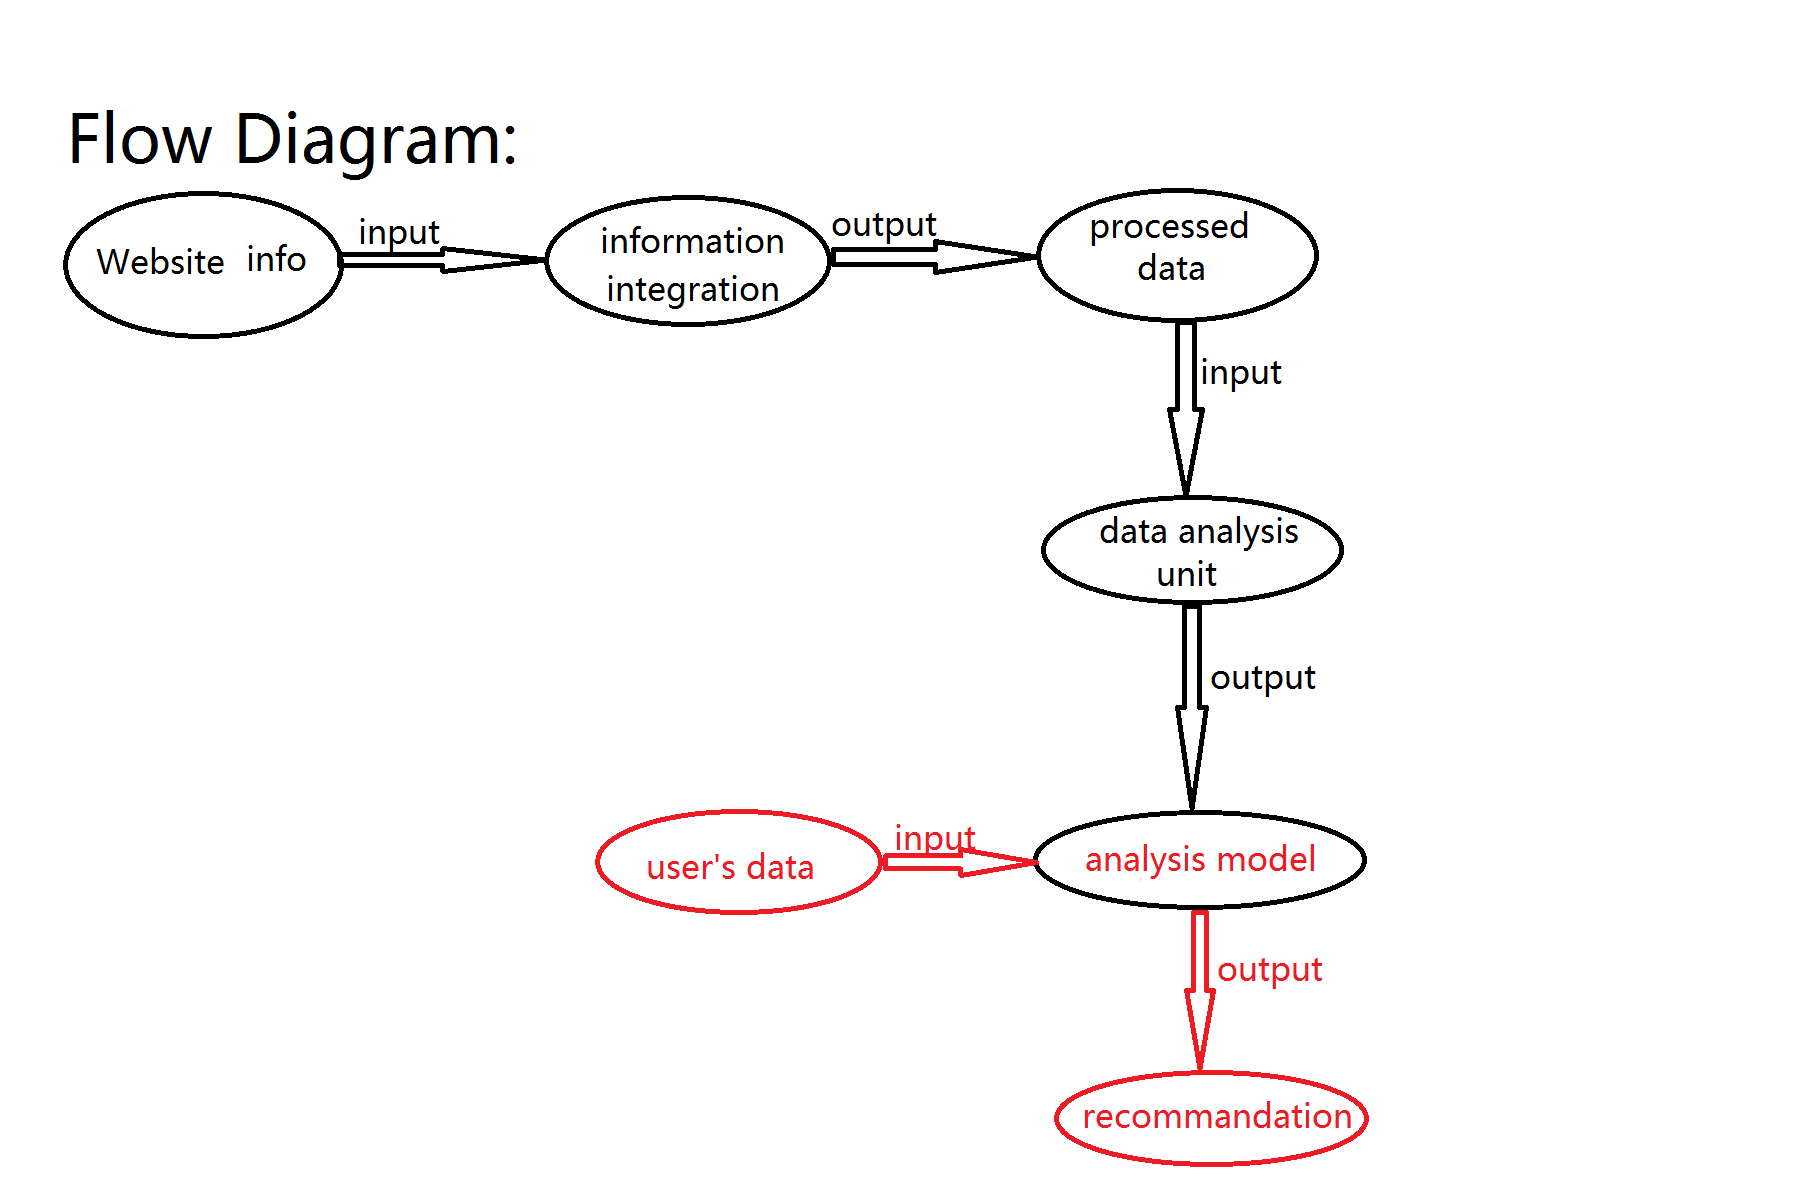
\includegraphics[width=0.4\textwidth]{512flowdiagram.png}
\caption{}
\end{figure}
\item{ High Level Pseudo Code System Description. }
\begin{itemize} 
\item{Information Integration Module: Integrating Unit(website-info)
We collect the houses' information of New Jersey from the website "weichert" using crawling to obtain the property information. Then we save the information to Excel files.
Return Processed data}

\item{Data Analysis Module: Data Analysis Unit(Processed data)
Pass Processed data to Data Analysis Unit, then process it through Regression Unit. The process procedure includes to uniform the file style, to remove the redundant information from the original dataset, to transform the non-digital information to digital information.
Deposit it to system database}

\item{User's Preference input()
Input User's preference}

\item{Regression Unit()
Rate user's input house, then give the prediction using linear regression on house's price. 
Form a suggestion feedback to users}
\end{itemize}
\item{Algorithms and  Data Structures. }
Algorithms and  Data Structures: First we use web crawling algorithm to stretch useful data from website. This algorithm works with website code and get different digital data from website. Secondly we process these data to table structure type which our data analysis unit could use. Finally, we use our model deal with digital data and output useful recommendations. 
\item{As to the data structure, we use list to save houses' information from the website, process the data using string, use data frame to achieve regression and price prediction.}
\item{The main algorithms used in our project are crawling to get the total information from the website, bubble sort which is used for sorting the house list according to the prices provided from the website and regression which is used for providing the standard of price prediction and providing similar houses from the system data-list.}
\end{itemize}

\begin{itemize} 
\item{  Flow Diagram Major Constraints.}

\begin{itemize} 
\item{ First integrity constraint: Houses data on the website must contain price, room numbers, year, area. }
\item{ Second integrity constraint: Input data to the data analysis unit must be table format with numbers. }
\end{itemize}
\end{itemize}
}


\subsection{Stage3 - The Implementation Stage. }\label{sec: 3 The Implementation Stage.}
%%%%%%%%%%%%%%%%%%%%%%%%%%%%%%%%%%%%%%%%%%%%%%%%%%%%%%%%%%%%%%%%%%%%%%%%%%%%%%%%%%%%%%%%%
\textnormal{
The programming language we use for this project is Python 2.7, the programming environment is Windows 64-bit.
%Building the corresponding relational tables, according to the proposed ER model described in the previous phase %enforcing the different integrity constraints.  
The deliverables for this stage include the following items:
\begin{itemize} 
\item{Data Snippet: See Fig.2}
\begin{figure}
\centering
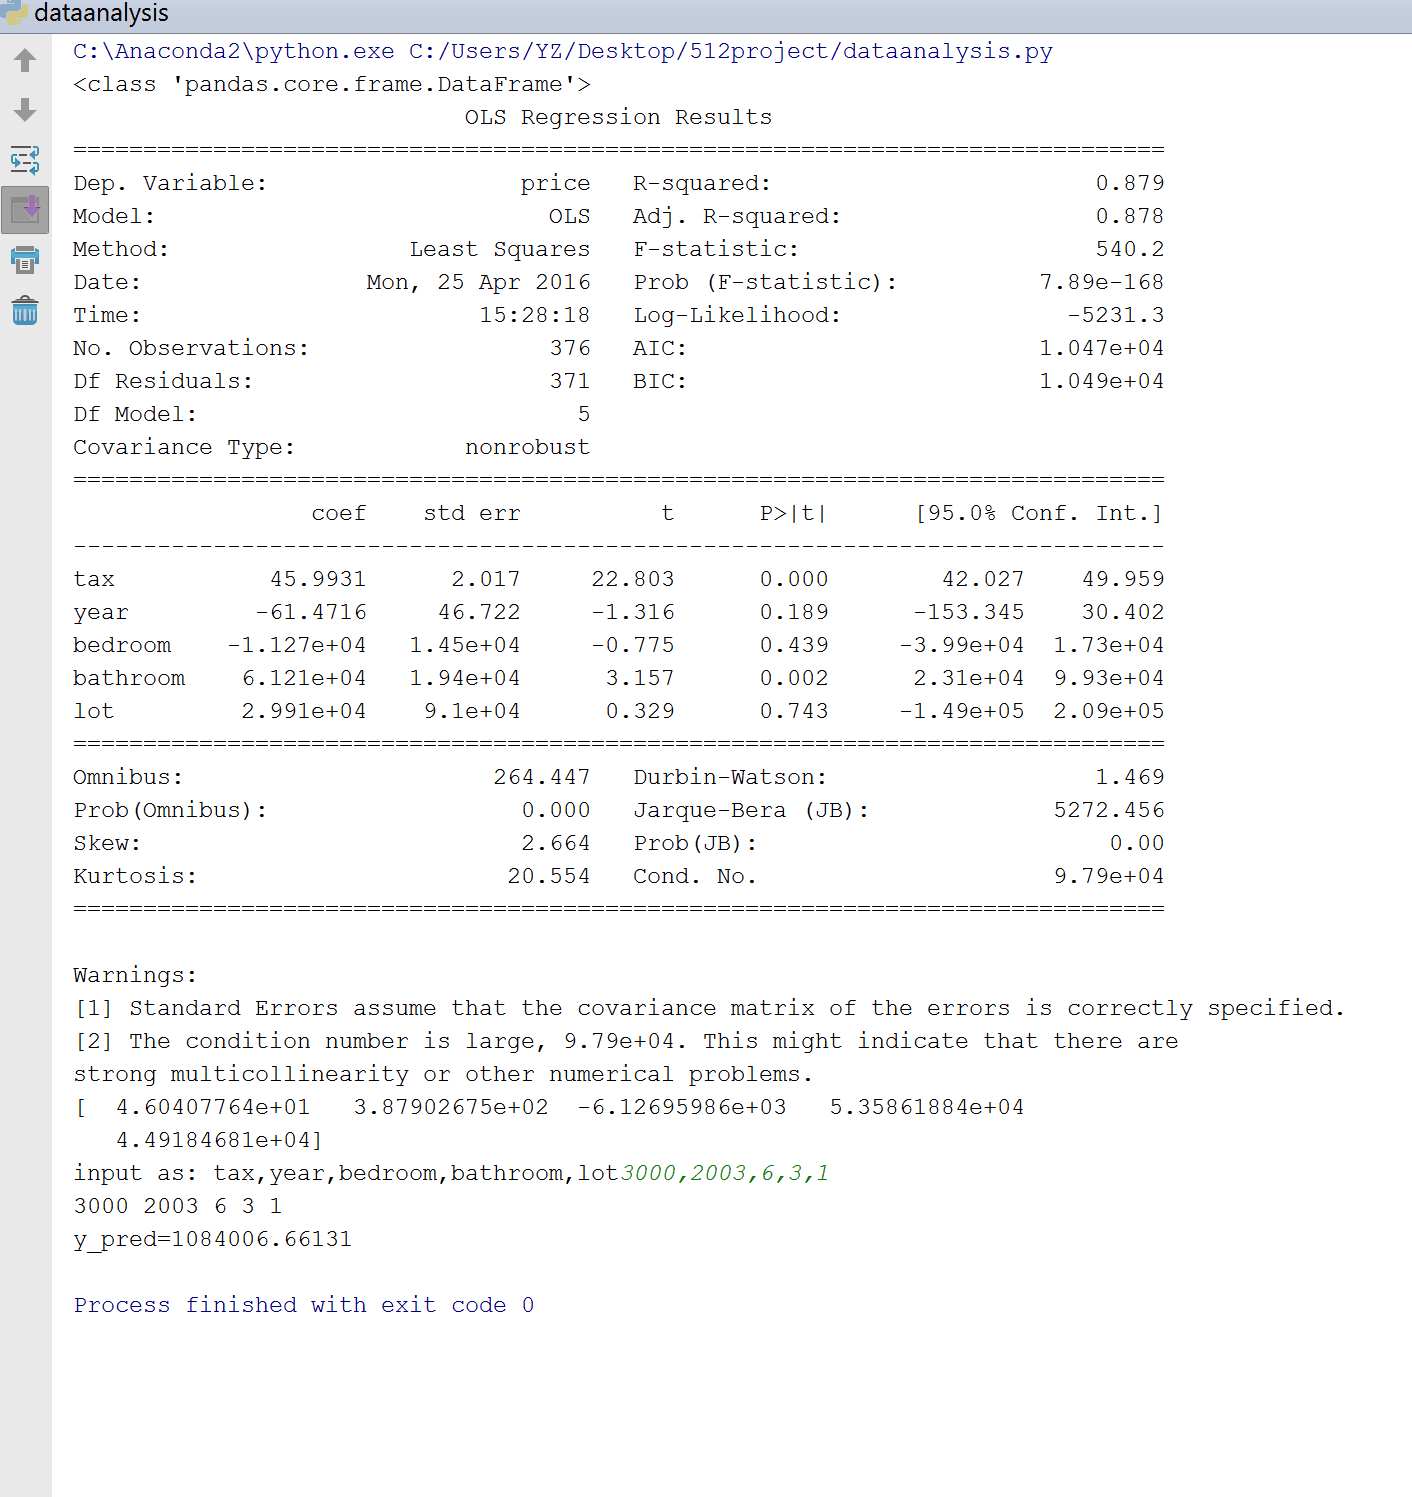
\includegraphics[width=0.5\textwidth]{RegressionPredictionOutput.png}
\caption{}
\end{figure}
%The SQL tables that represent the ER project model, along with at least 3-5 rows of concrete data per table.
\item{Regression and Prediction: See Fig.3}
\begin{figure}
\centering
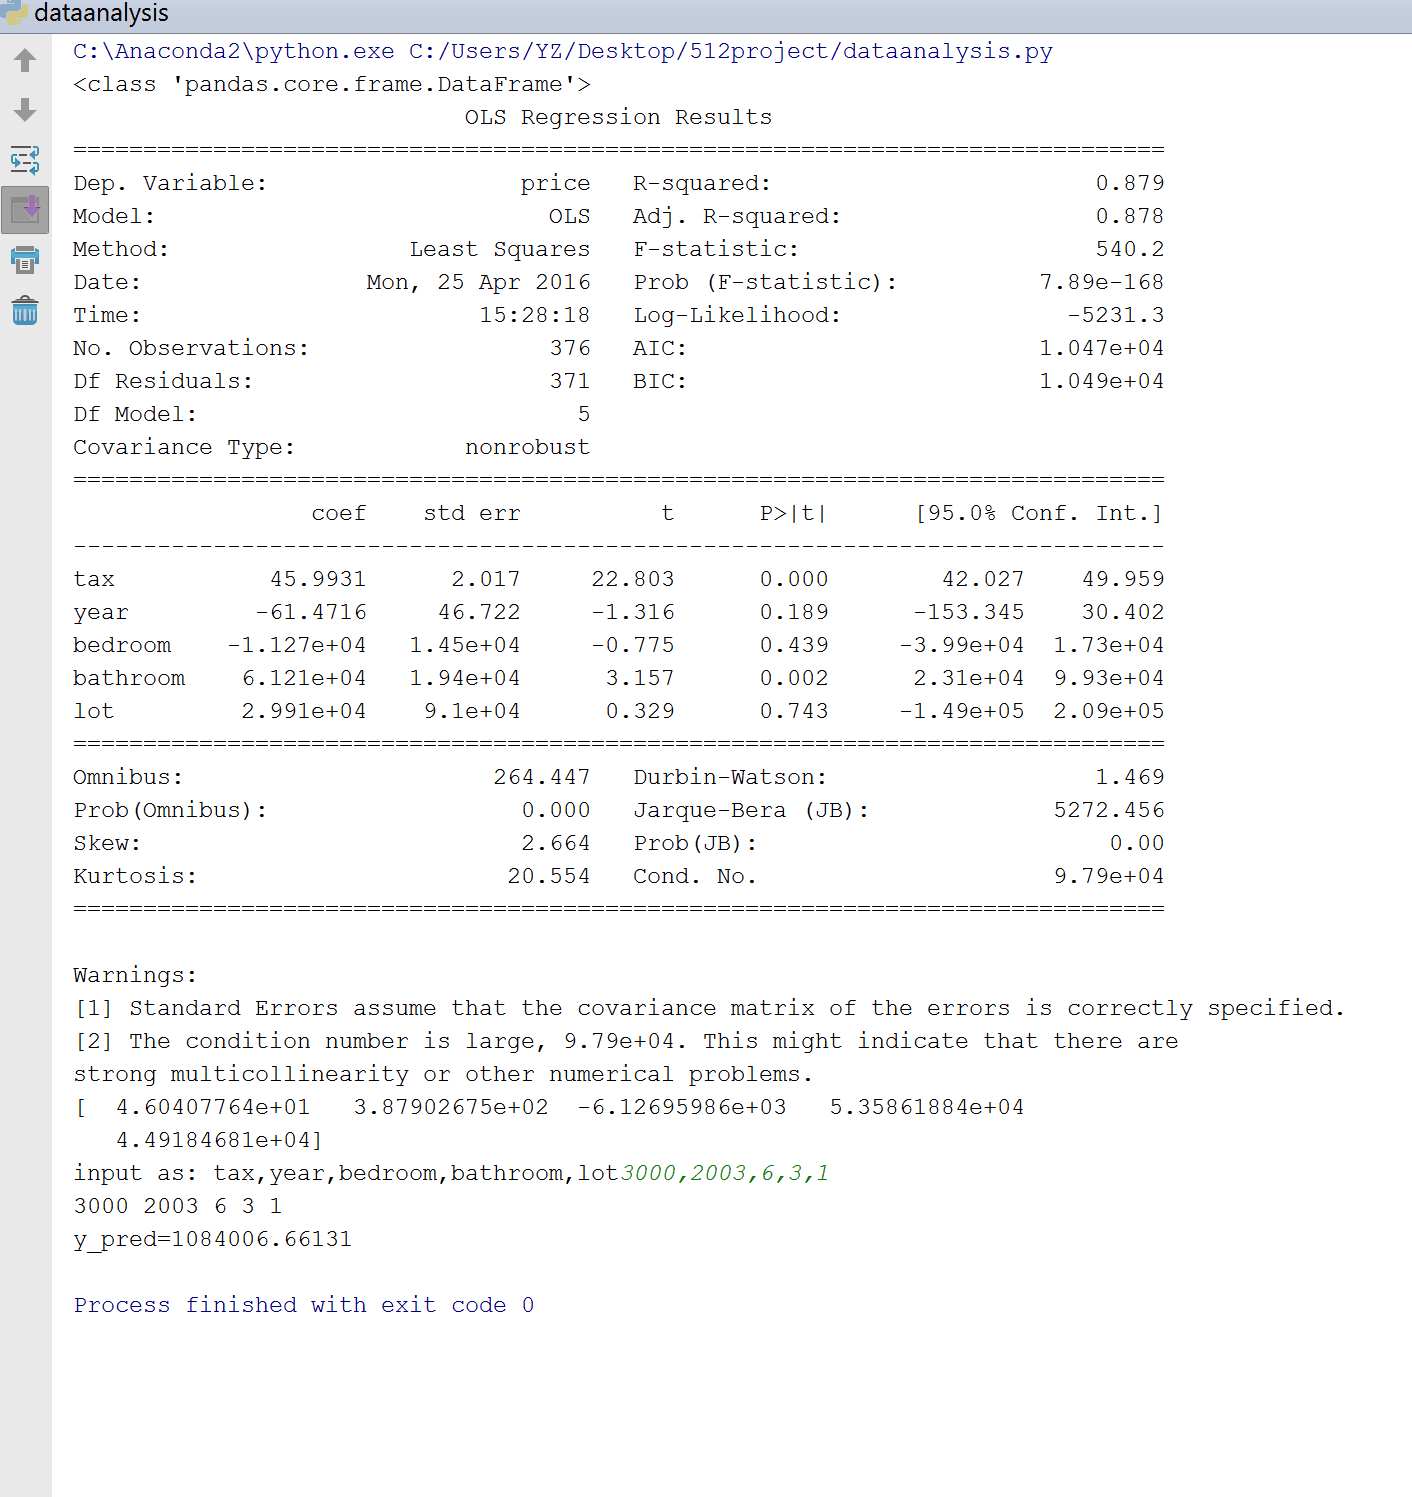
\includegraphics[width=0.5\textwidth]{RegressionPredictionOutput.png}
\caption{}
\end{figure}
%The normalization steps for each table, along with explanations/justifications of each normalization step.
\item{Datacrawling: See Fig.4-6}
\begin{figure}
\centering
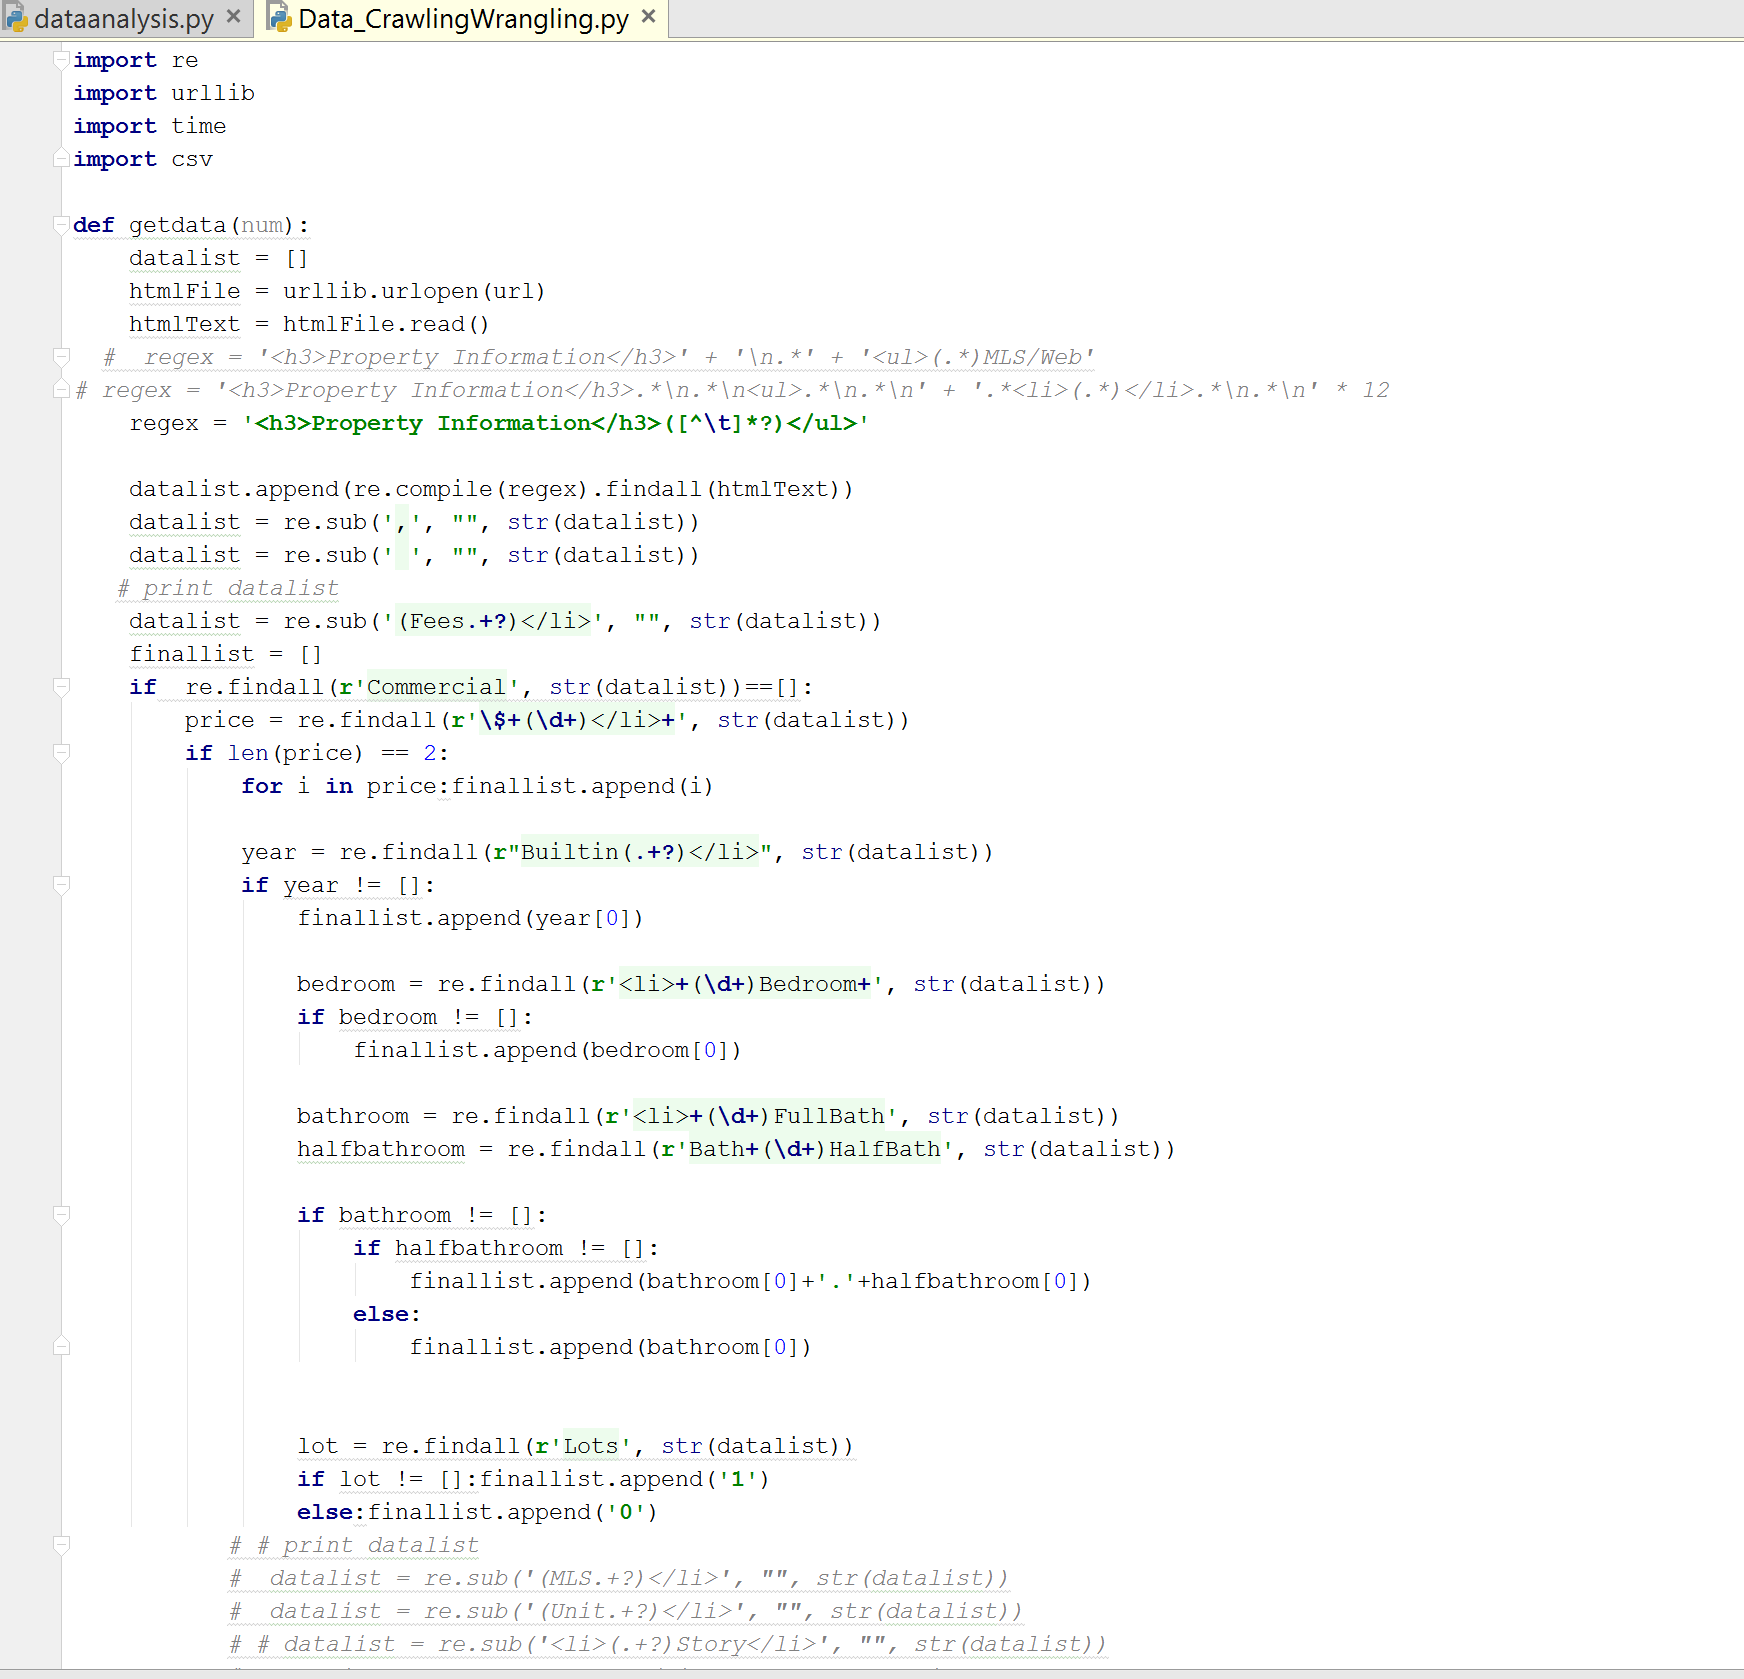
\includegraphics[width=0.5\textwidth]{datacrawling1.png}
\caption{}
\end{figure}
\begin{figure}
\centering
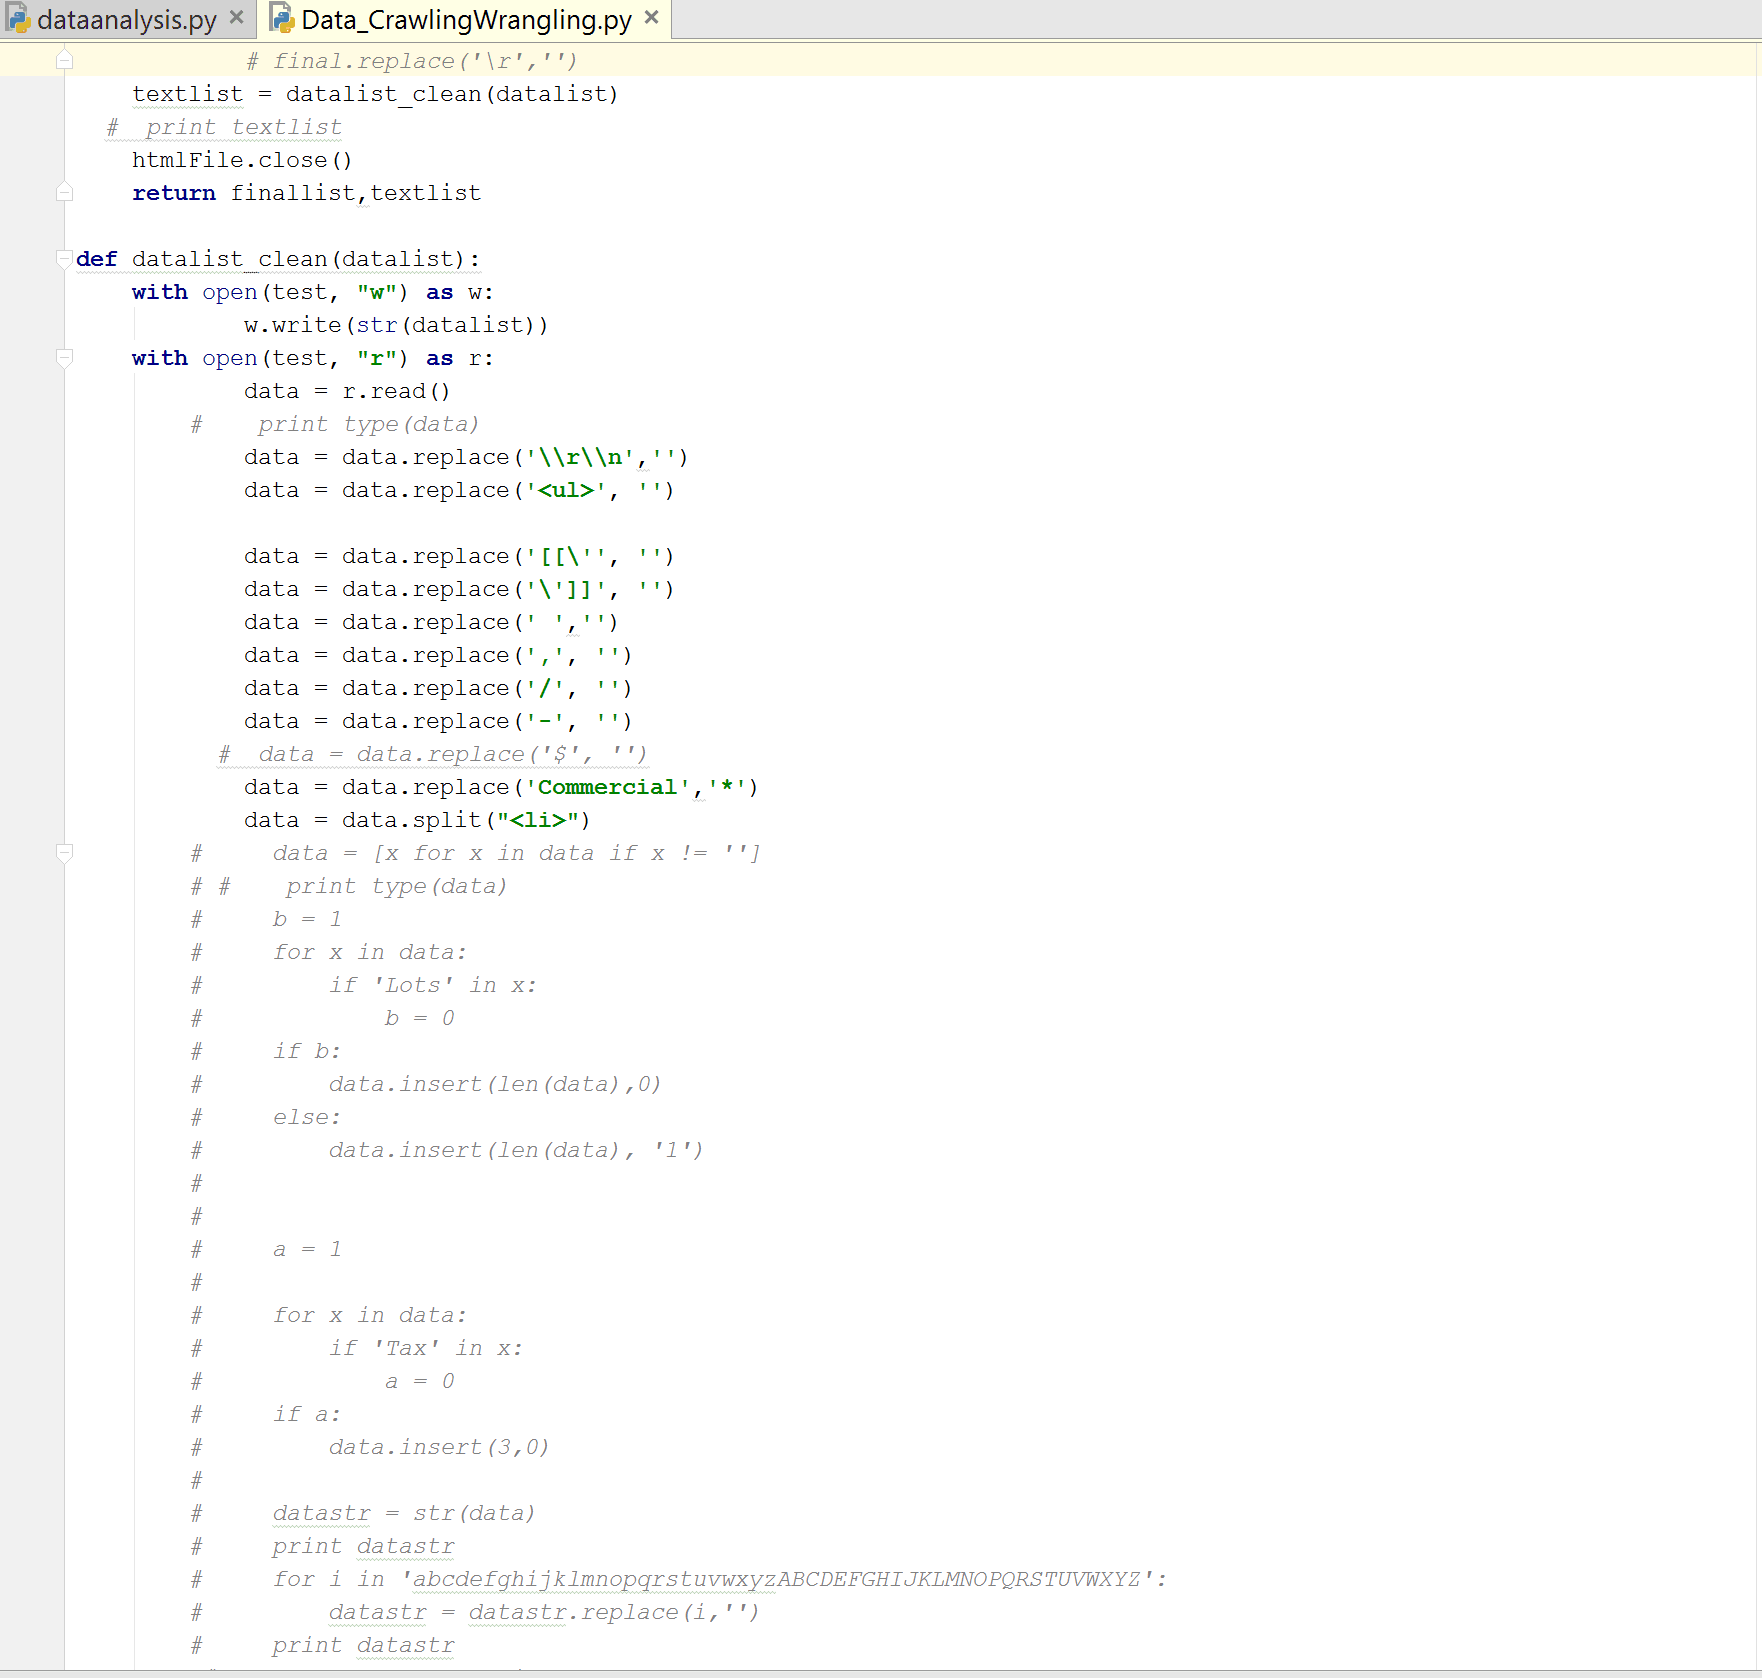
\includegraphics[width=0.5\textwidth]{datacrawling2.png}
\caption{}
\end{figure}
\begin{figure}
\centering
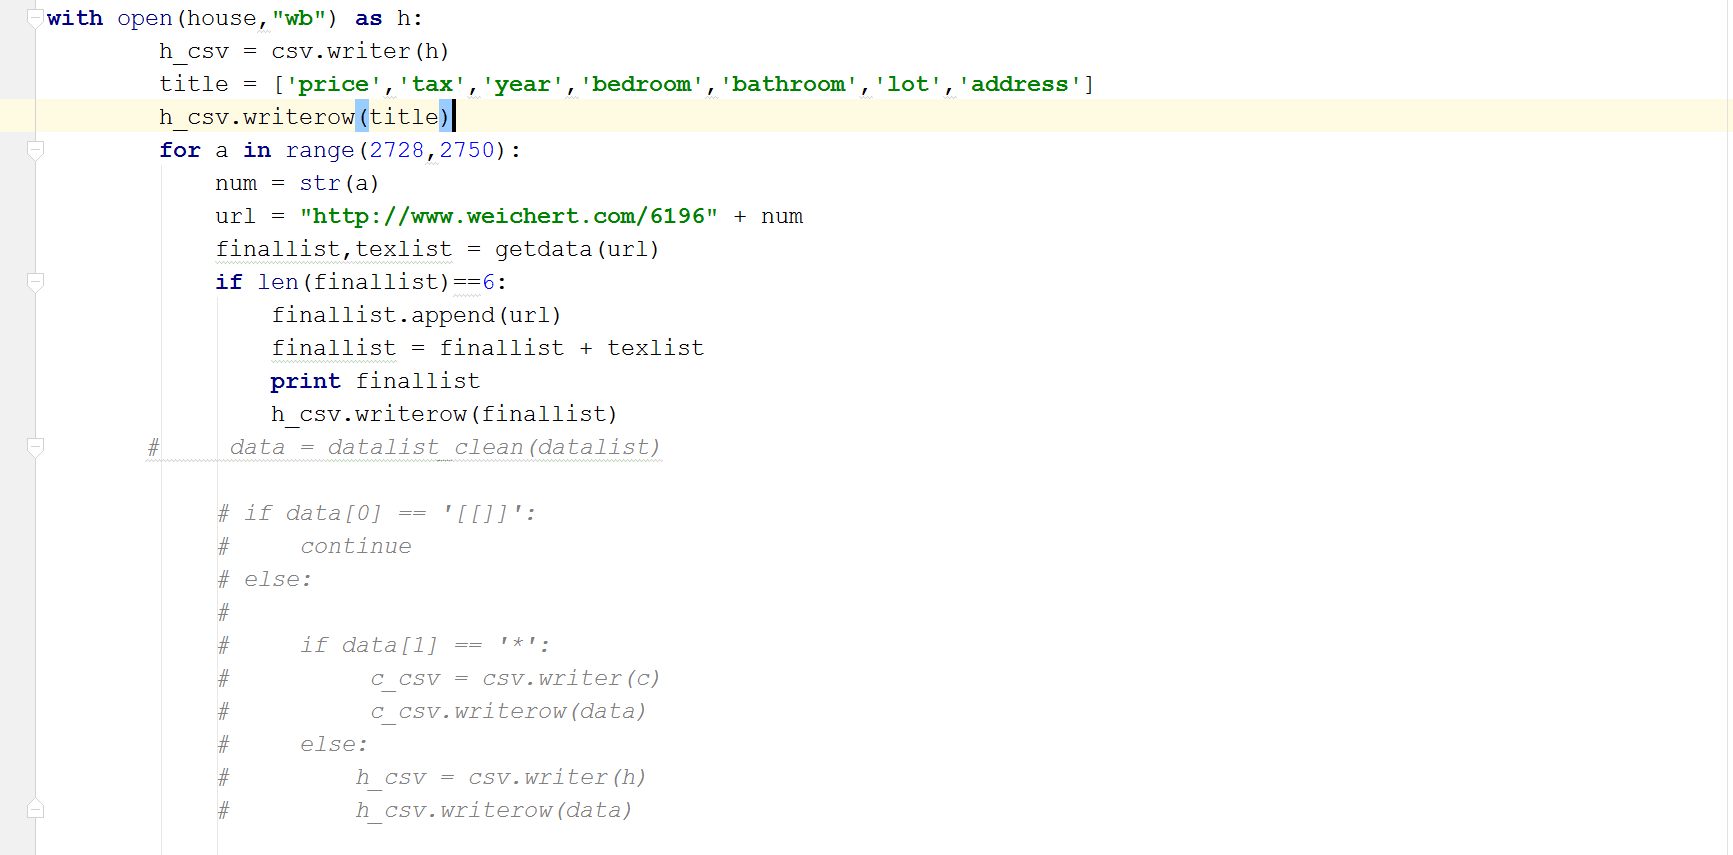
\includegraphics[width=0.5\textwidth]{datacrawling4.png}
\caption{}
\end{figure}
\item{DataAnalysis: See Fig.7-8}
\begin{figure}
\centering
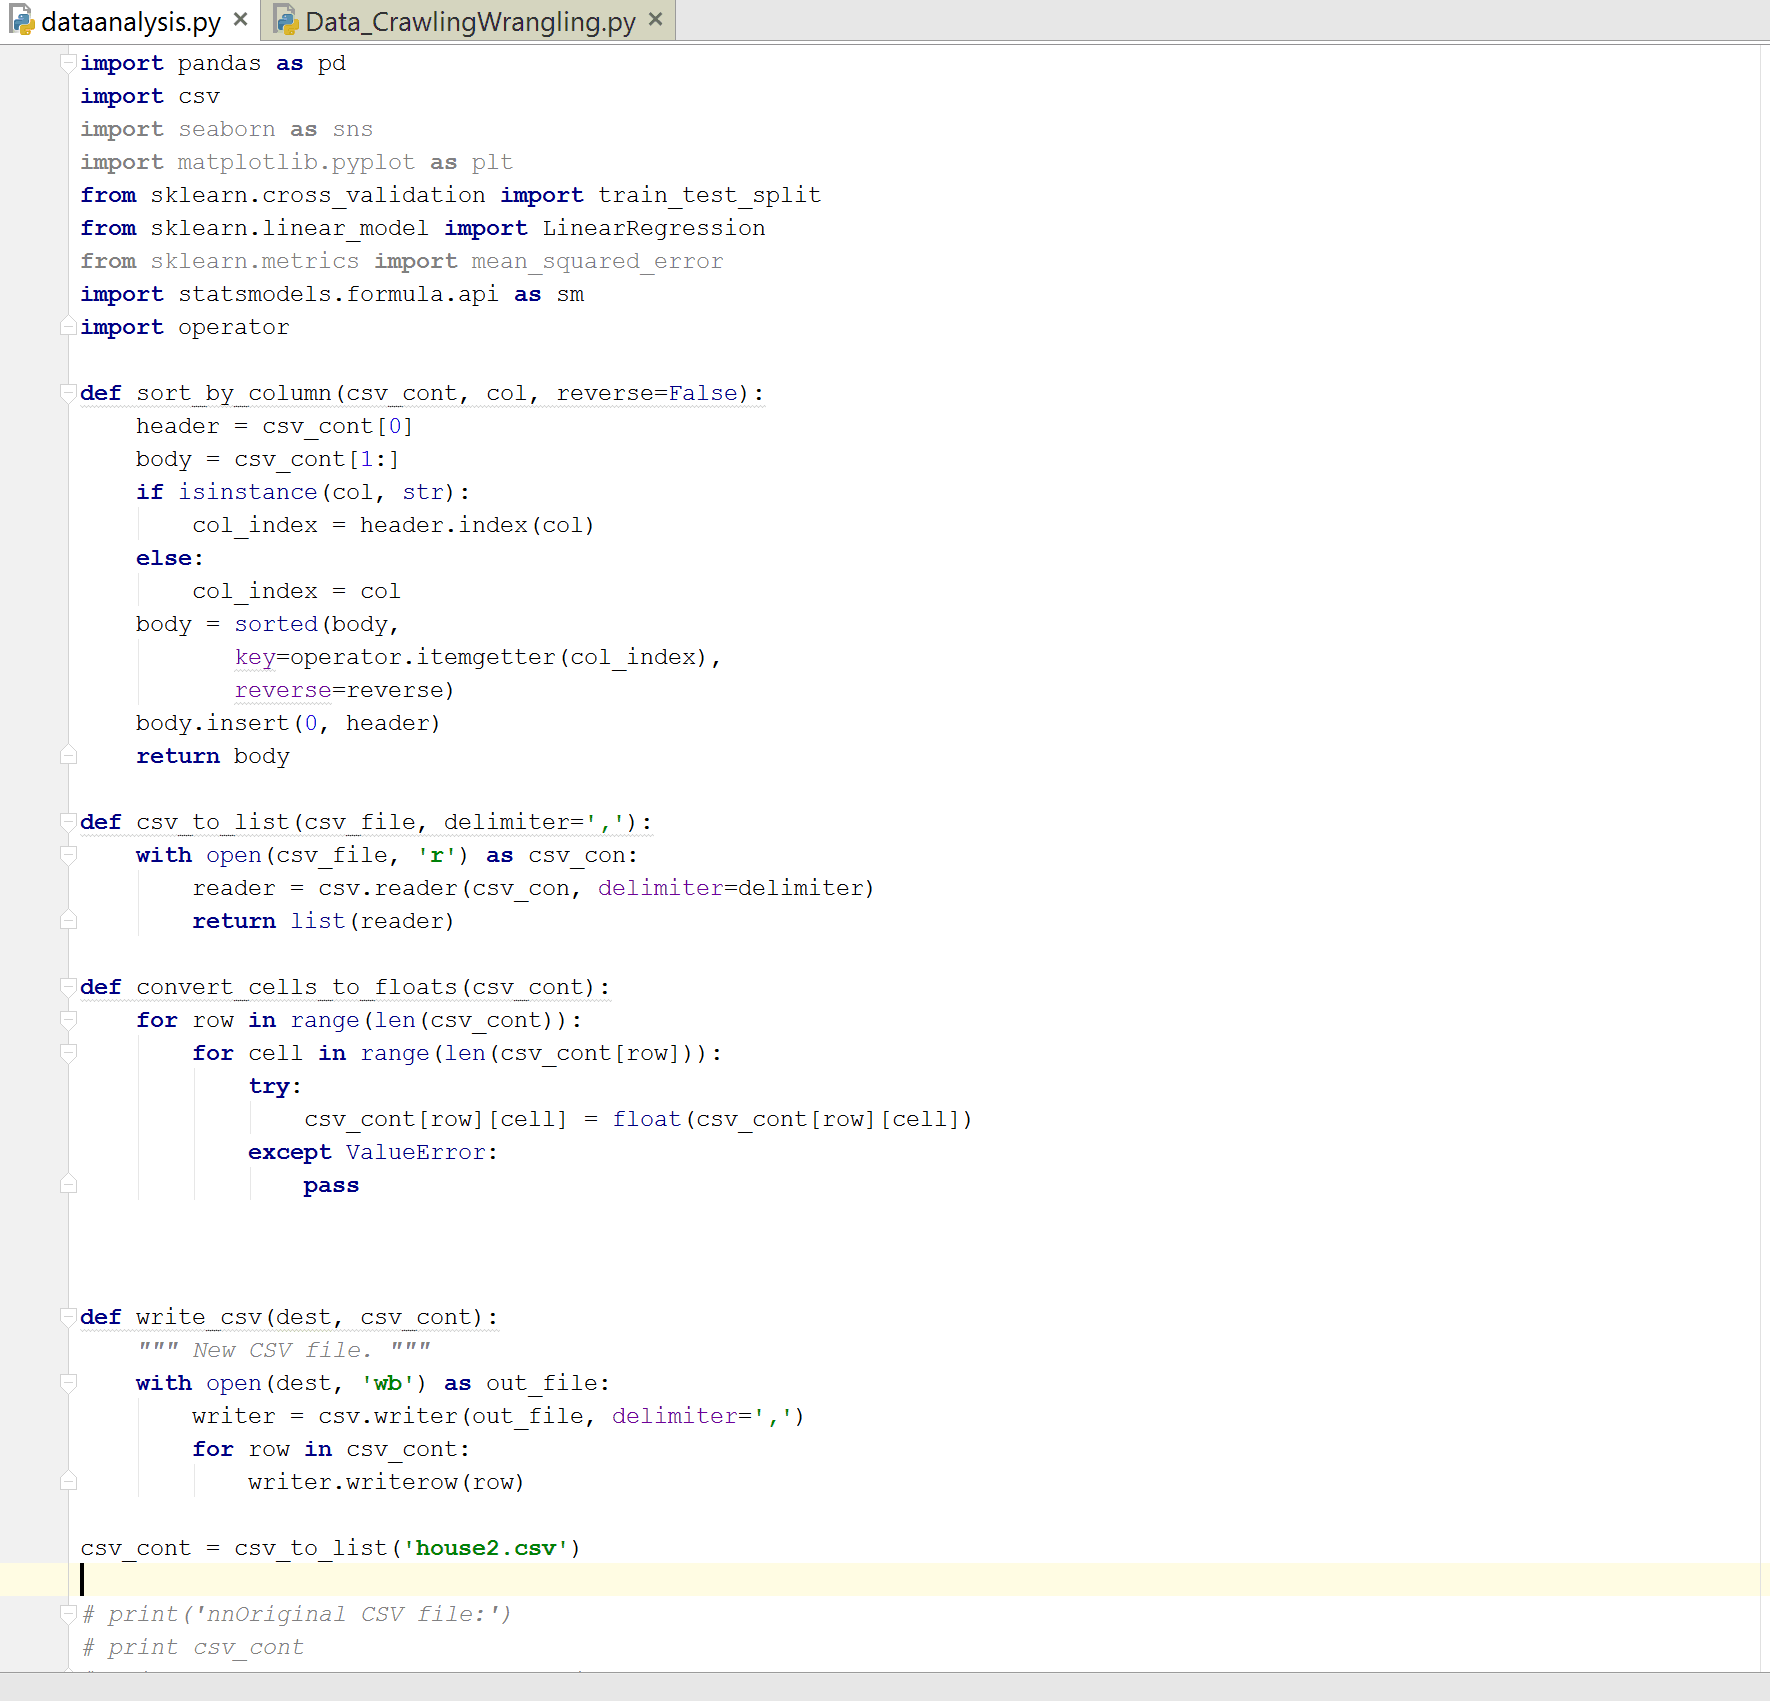
\includegraphics[width=0.5\textwidth]{DataAnalysis1.png}
\caption{}
\end{figure}
\begin{figure}
\centering
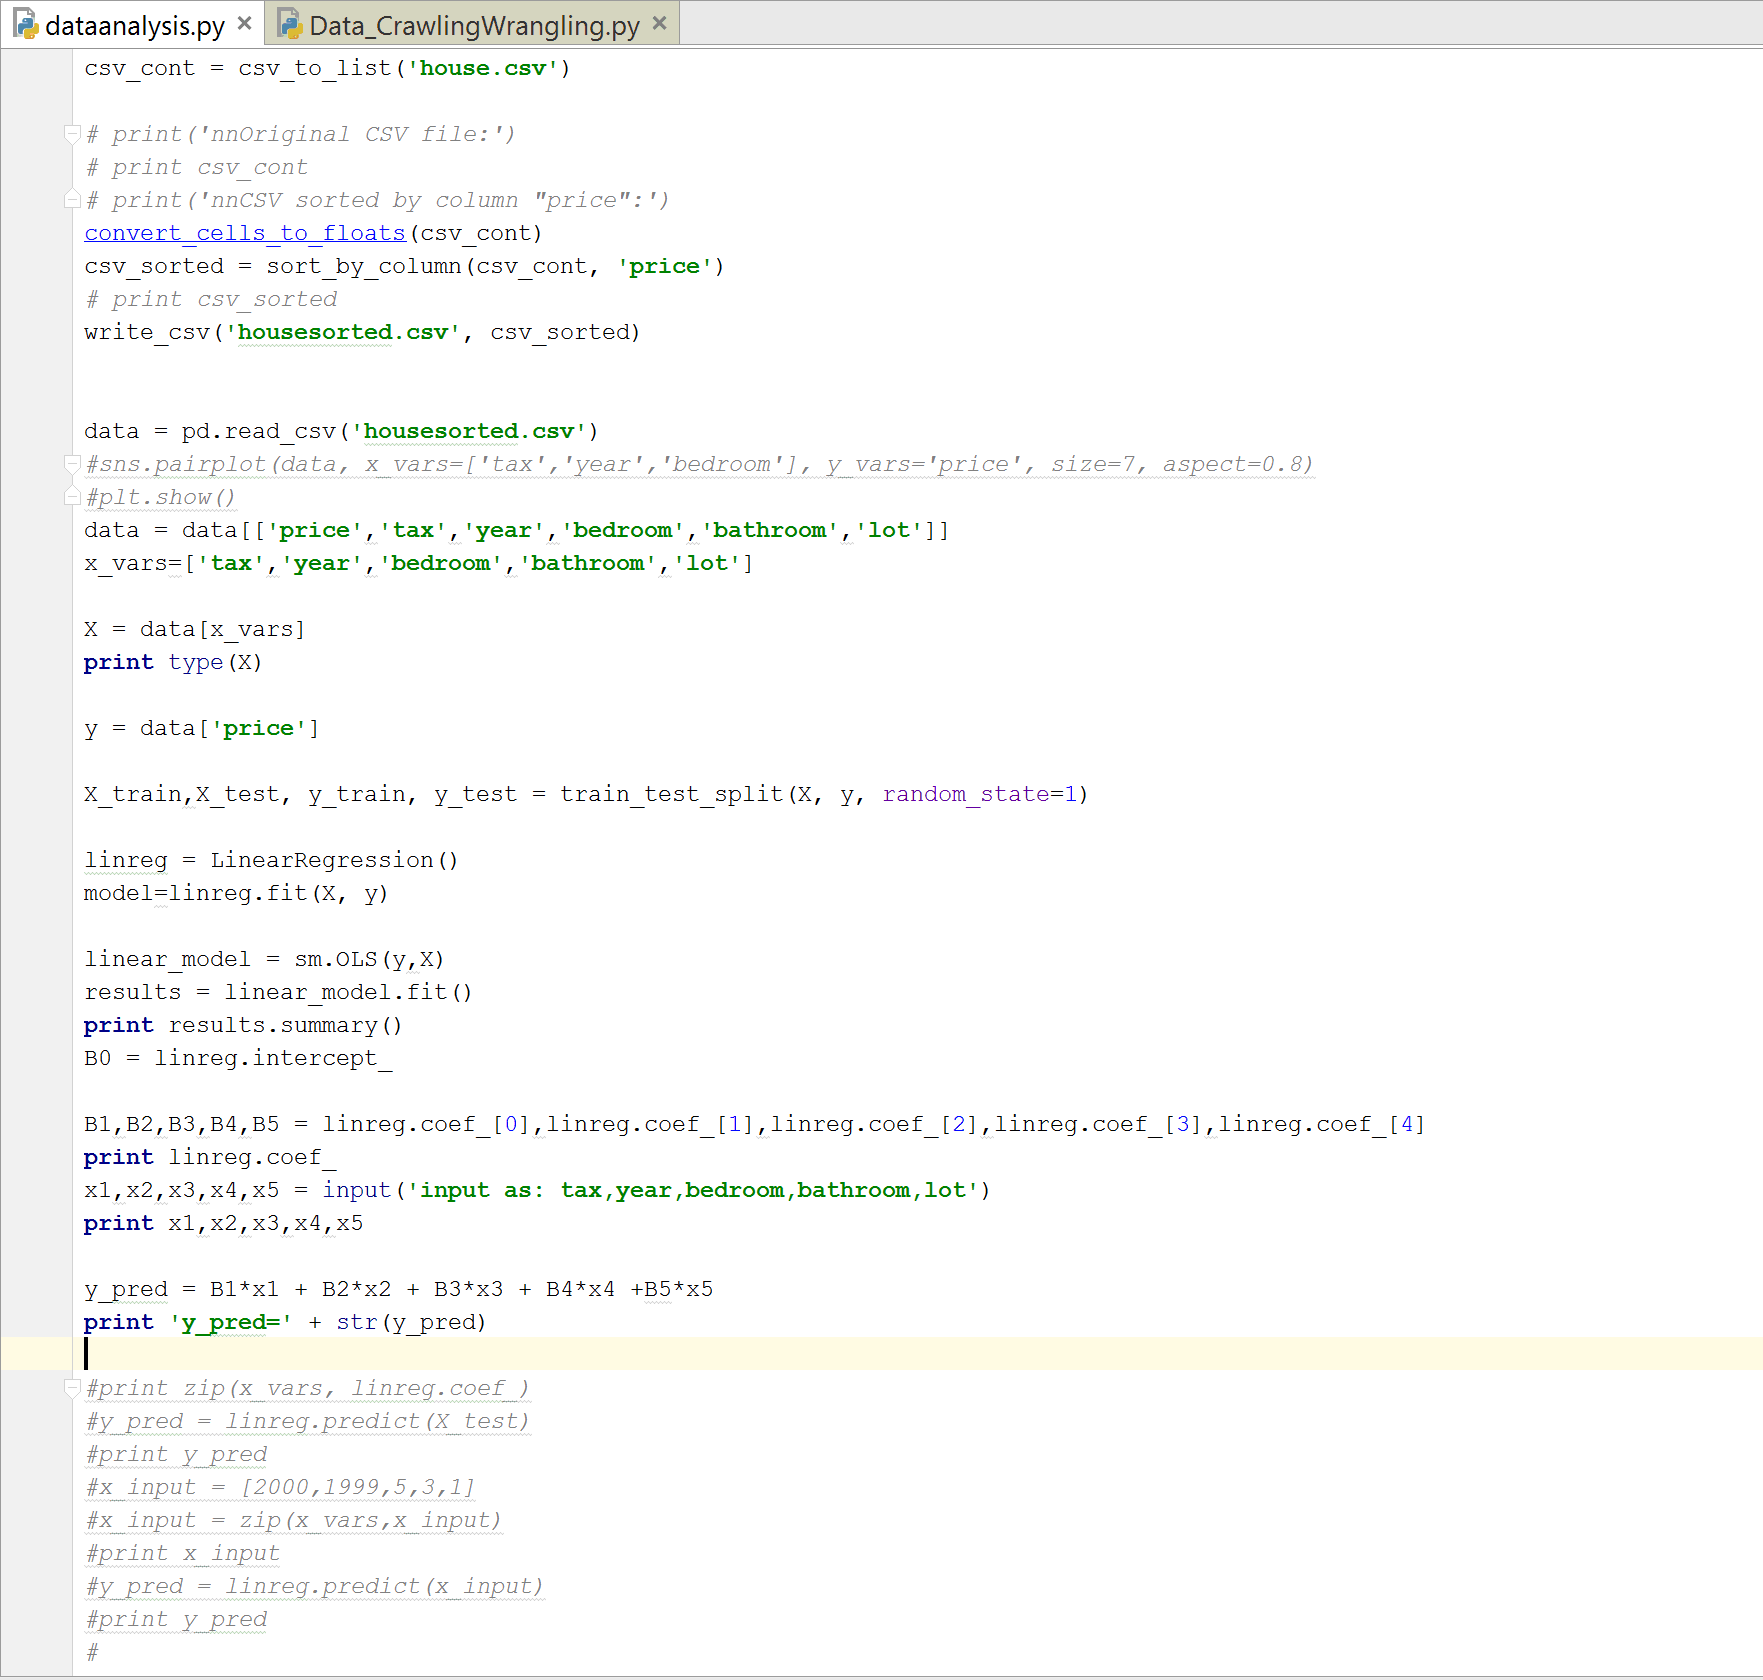
\includegraphics[width=0.5\textwidth]{DataAnalysis2.png}
\caption{}
\end{figure}
%The SQL table after the normalization steps (showing all table attributes).
\item{}
Demo and sample findings
%The SQL statements used to create the SQL tables, including the required triggers as well as the integrity constraints. At %least 2 triggers and 2 of each of the following constraint types have to exist in the project tables overall: 
\begin{itemize} 
\item{}
	Data size: 1MB;  Disk Resident: 10MB;  
\item{}
	 We collect houses' information from "weichert", calculate the prediction price through multiple linear regression.
	 After collecting all the information from the website, we find out that the built-year of houses have no effects on houses' prices. And this is weird, because in common sense, the elder the house is, the lower the price will be, considering higher cost on maintenance, lower security standard. Maybe the website does not put the built-year into the calculation standard.
%Whether some users will be denied access and/or updates to some data according to their roles (for example: student1 %can not access other students' ' grades, so a violation error pops up upon that action. Another example: a sales person %can see an item price, but can not change it, since only a manger can, also a violation error pops up upon that update %attempt).
\end{itemize}
\end{itemize}
}


\subsection{Stage4 -	User Interface. }\label{sec: 4. User Interface.}
%%%%%%%%%%%%%%%%%%%%%%%%%%%%%%%%%%%%%%%%%%%%%%%%%%%%%%%%%%%%%%%%%%%%%%%%%%%%%%%%%%%%%%%%%%%%%%%%%%%%%%%%%%

Please insert your deliverables for Stage4 as follows:
\begin{itemize} 
\item{Unzip the interface web page and related data into a directory, run the command "python -m SimpleHTTPServer 8000" (if using python 2) or "python -m http.server 8000"(if using python 3) in the directory, then use a web browser and navigate to localhost: 8000/ house data filter.html. The initial screen shot:
\begin{figure}
\centering
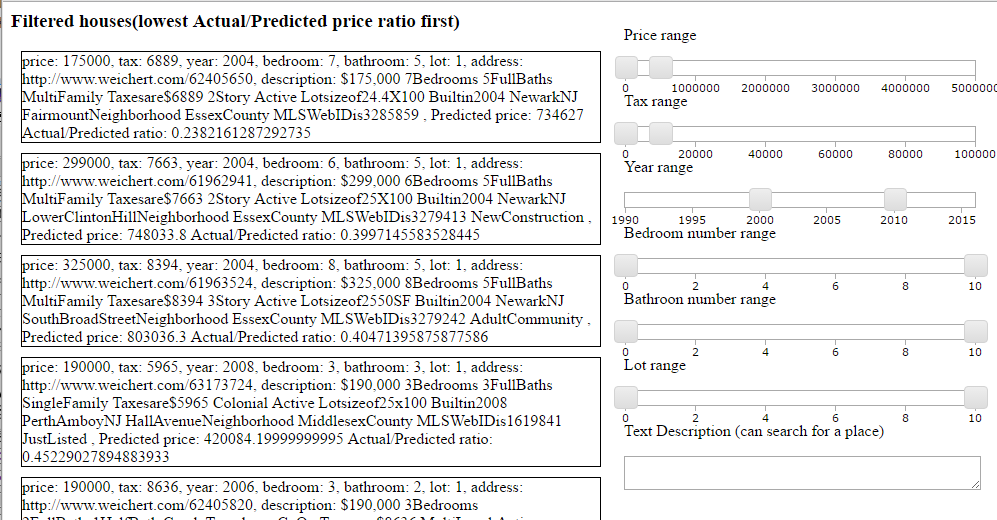
\includegraphics[width=0.5\textwidth]{houseinitial.png}
\caption{}
\end{figure}

	
\item{Two different  sample navigation user paths through the data exemplifying the different modes of interaction and the corresponding screen shots. 

1. The user wants to find cheap small houses, so slide the bedroom, bathroom, price and tax sliders to the left, then the web page will display the houses that seem like deals according to the actual price to predicted price ratio. The predicted price is calculated with the coefficients obtained from linear regression.

\i\begin{figure}
\centering
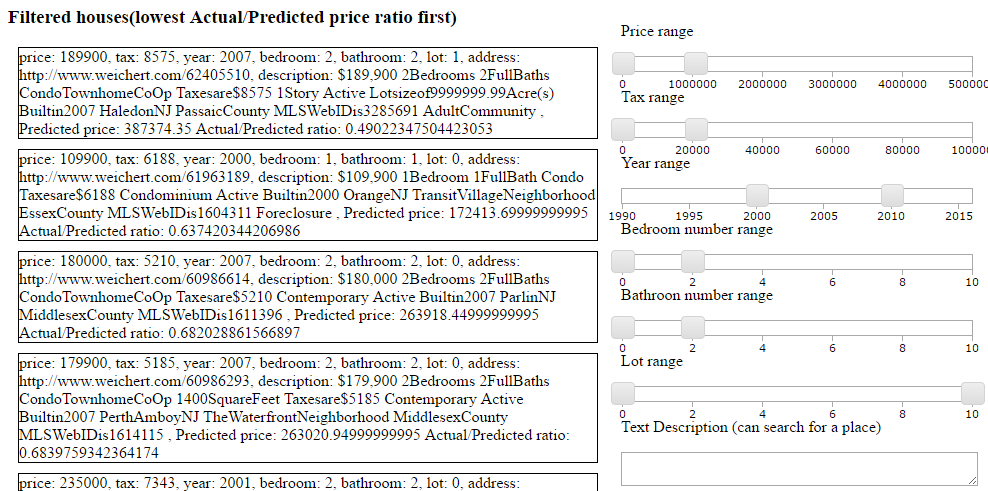
\includegraphics[width=0.5\textwidth]{housesmall.png}
\caption{}
\end{figure}

2. The user wants to find any houses that are deals in the Edison region, so type the text "Edison" (case sensitive) into the Text description search box, and slide all sliders as wide apart as possible. The top houses displayed are the ones that seem to be deals according to the linear regression.

\begin{figure}
\centering
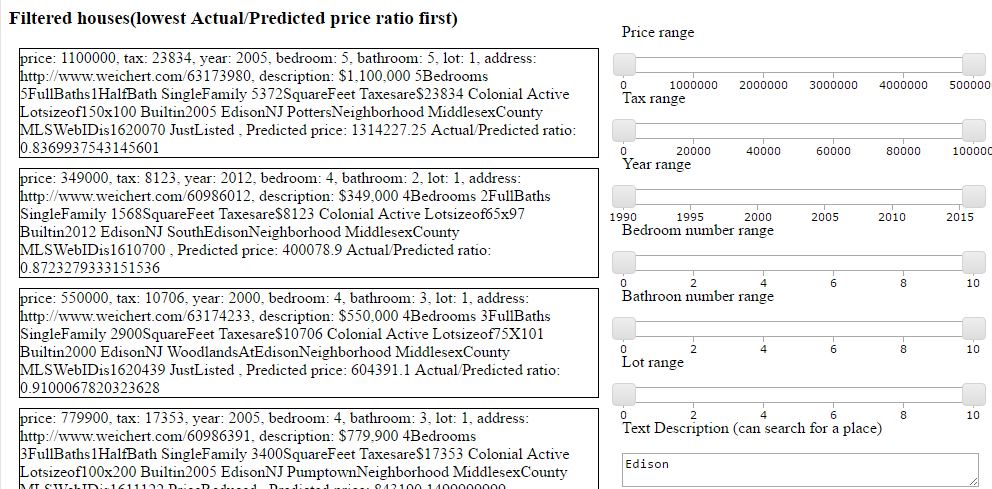
\includegraphics[width=0.5\textwidth]{houseedison.png}
\caption{}
\end{figure}

}
\item{}
	The error messages popping-up when users access and/or updates are denied (along with explanations and examples):
	\begin{itemize} 
	\item{The error message: There are no access denied error messages, because the data gathering/storing and the user interface are different parts in our application. The user interface has all access to data already scraped from the Web.}
	\item{The error message explanation (upon which violation it takes place): }
	The houses display being empty means that the request cannot be met within the current data set.
	\item{The error message example according to user(s) scenario(s): }
	If the user inputs a place name incorrectly (for example, type "Edison" as "Eddison") then most likely there will be no results displayed. What's more, since the result is updated in real time for every character of text, the user can notice the mistake immediately when he types "Edd". 
	 \end{itemize}
\item{}
	The information messages or results that pop-up in response to user interface events.
	\begin{itemize} 
	\item{The information message: }
	The "message" is the left side's houses display area being empty.
	\item{The information message explanation and the corresponding event trigger }
	Because the user starts typing "Edison" as "Eddison" in the text search box, the houses display becomes empty because "Edd" doesn't match any data records.
	\item{The error message example in response to data range constraints and the corresponding user's scenario }
	If the user inputs conditions that cannot be met, the displayed houses area will immediately be empty, and the user can simply correct it and do not need to click on a pop-up.
	The interface showing no houses match a mistake in input: 
	\begin{figure}
\centering
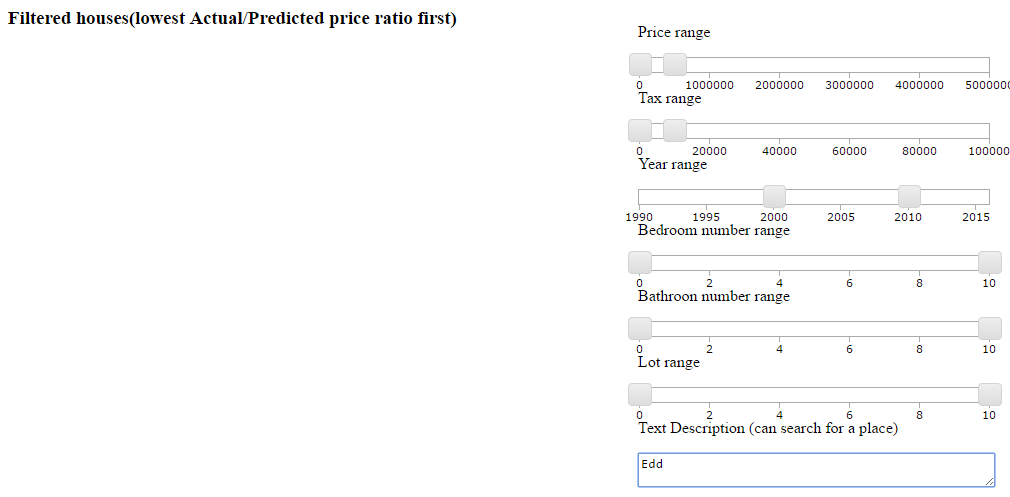
\includegraphics[width=0.5\textwidth]{housemistake.png}
\caption{}
\end{figure}
	 \end{itemize}
\item{}
	The  interface mechanisms that activate different views.
	\begin{itemize} 
	\item{The interface mechanism: }
	There is only one view, and the filtering of information is controlled by sliders and search boxes.
	 \end{itemize}

}


\section{Project Highlights.}\label{sec:7. Project Highlights.}
%%%%%%%%%%%%%%%%%%%%%%%%%%%%%%%%%%%%%%%%%%%%%%%%%%%%%%%%%%%%%%%%%%%%%%%%%%%%%%%%%%%%%%%%%%%%%%%%%%%%%%%%%%

\begin{itemize} 
\item{}
Our project aims at building a house-buying system for users like house-seekers, landlords, leasing agencies. The recommendation system provides predictions on house's prices according to all the preferences. The system database are built from the website "Weichert", and price prediction is fulfilled using multiple linear regression which ensures the accuracy of the system. Upon using the system interface, users can get the similar houses directly when they move the preference sliders, and it's simple to use.

\begin{enumerate}
\item{}
Title: House buying system(Yi Zhong, Qingqiao Hu, Qi Dong)
\item{}
Project Goal: Building a recommendation system on house sale.
\item{}
Outline of the presentation: 
\item{}
Description: Our project is based on the information from “Weichert”, a website of house renting or buying, and we focus on the houses of New Jersey. We collect the house's information, and save them to our system database. We use linear regression to give prediction to the house price according to the preferences provided by users, and provide the concrete property information of houses for users to choose from. 
 √
\item{}
Pictures are included in stage 4.
\item{}
Project Stumbling Blocks: Information collection, Data processing, Linear Regression, UI Design                                
\item{}
Future Extensions: Expanding the System Database to the US, even the world, Providing more preferences for users to choose from, Building a virtualization of the houses, so that users can get a clear view of similar houses according to the dynamic graph
\item{}
References: Weichert
\end{enumerate}

}


\bibliographystyle{IEEEtran}
%\bibliography{IEEEabrv,bib_queyroi_abello2013}
%\bibliography{bib_queyroi_abello2013}

\end{document}


